\chapter{Graphical Abstracts: One Image for One Contribution}

Zhou, a doctoral student working in satellite remote sensing and deep learning, has just received an acceptance letter for her manuscript. At the bottom of the email, the editorial office adds one final requirement: within a week, submit a graphical abstract to appear in the online table of contents (TOC) and at the top of the article page. To Zhou, the task sounds trivial. She opens her manuscript folder, selects Figure 1---an encoder--decoder network diagram with skip connections, channel dimensions, attention blocks, and a loss equation---scales it down proportionally, and uploads the exported image.

Two days later, the technical editor returns the file with a two-sentence note: ``This diagram shows the internal architecture of your network, not the contribution of your study; and when scaled to table-of-contents size, the text is illegible.''

Many authors asked for a graphical abstract for the first time step into the same trap: either they shrink a method diagram (Figure 1) from the paper, or they cram four or five result plots into one frame like a miniature poster. Specialists in the exact sub-field do not need the thumbnail, while readers browsing the table of contents from neighboring areas cannot tell in five seconds what problem the paper addresses or what it found. This chapter shows how to design a single image that communicates one research contribution and its essential boundary conditions clearly and conservatively under strict size and viewing-time constraints.

\section{What a Graphical Abstract Must Answer}

A graphical abstract is a single figure placed in an online table of contents, search listings, and the top of an article page. Within the three to eight seconds a reader spends scanning a table of contents, the image should answer three linked questions---\textbf{``Does this paper address a problem relevant to my work? How did the authors approach it? What bounded finding did they establish?''}

To accomplish that job, a graphical abstract needs to convey only a three-part chain: \textbf{Question --- Method --- Finding and Limits}. It does not catalog kernel sizes layer by layer, list hyperparameters or secondary ablations, or reproduce statistical plots with error bars and significance asterisks.

Before sketching a layout, distinguish the graphical abstract from three other visual formats that are often confused with it:

\begin{center}\footnotesize
\setlength{\tabcolsep}{3pt}
\renewcommand{\arraystretch}{1.15}
\begin{tabularx}{\linewidth}{@{}>{\raggedright\arraybackslash}p{23mm}>{\raggedright\arraybackslash}p{25mm}YY@{}}
\toprule
\textbf{Figure format} & \textbf{Placement and viewing time} & \textbf{Primary audience and core job} & \textbf{Common misuse and pitfalls} \\
\midrule
Paper Figure 1 (method or framework) & Inside the Methods section; studied for several minutes with the text & Peers already reading the full paper; explains module wiring, tensor dimensions, data flow, or experimental groups & Shrinking Figure 1 directly into a graphical abstract, showing internal wiring without the research question or finding \\
Graphical abstract (TOC graphic) & Online table of contents, search listings, and article top; $3\text{--}8$ seconds & Cross-disciplinary readers browsing an issue; conveys ``question--method--finding and limits'' to guide reading decisions & Packing in multi-panel data plots, parameter tables, or tiny legends that blur together at TOC thumbnail size \\
Visual abstract & Journal social-media feeds and summary cards (common in clinical journals); a few seconds & Researchers and clinicians scrolling social feeds; uses a multi-column card template with key metrics for sharing & Copying social-media slogans into a journal TOC graphic or omitting study population and scope restrictions \\
Conference poster & Exhibit board; discussed in person for $2\text{--}5$ minutes & Conference attendees; presents background, workflow, primary data plots, and conclusions (see Chapter 12) & Compressing a multi-column poster into a graphical abstract, shrinking font height tenfold until text is unreadable \\
\bottomrule
\end{tabularx}
\end{center}

Does adding a graphical abstract guarantee more views or citations? Empirical studies have reached different conclusions depending on the setting. Pferschy-Wenzig et al.\ (2016) compared articles published with and without a graphical abstract in \textit{Molecules} and found that, within their sample and observation window, papers with a graphical abstract did not show higher citations, abstract views, or downloads than papers without one (consult the original paper for sample construction and analysis methods). Conversely, in a prospective, case-control crossover study of surgical papers shared on social media, Ibrahim et al.\ (2017) found that tweets paired with a visual abstract received more impressions, retweets, and article visits than plain-text tweets.

Together, these findings point to a clear rule: \textbf{never assume that a graphical abstract will raise citations, and never inflate claims to catch the eye.} Its real value is \textbf{accurate rapid comprehension}---helping the right readers recognize your work in seconds while stating the conditions under which the conclusion holds.

\section{Read the Journal's Rules First: Aspect Ratio Before Composition}

Many researchers draw a figure first and check journal guidelines only when uploading files, only to find that the canvas shape is wrong: a square diagram forced into a $5:2$ banner either leaves wide blank margins or squashes elements vertically.

In graphical-abstract production, \textbf{journal format rules are not a final export setting; they are your first compositional constraint}. Publishers differ in aspect ratio, minimum pixel dimensions, fonts, and content rules. Table~\ref{tab:ch10-01-rules} and Figure~\ref{fig:ch10-01} summarize rules from three representative publishers (Elsevier, Cell Press, and ACS).

\begin{table}[htbp]\centering\footnotesize
\setlength{\tabcolsep}{3pt}
\renewcommand{\arraystretch}{1.15}
\caption{Graphical-abstract and TOC-graphic rules across three representative publishers (compiled from official author pages accessed October 2026; individual journals under the same publisher may differ, so always verify the target journal's current page before submission).}\label{tab:ch10-01-rules}
\begin{tabularx}{\linewidth}{@{}>{\raggedright\arraybackslash}p{23mm}>{\raggedright\arraybackslash}p{28mm}>{\raggedright\arraybackslash}p{26mm}Y@{}}
\toprule
\textbf{Publisher / example venue} & \textbf{Dimensions and aspect ratio} & \textbf{Resolution, fonts, and file types} & \textbf{Core layout and content rules} \\
\midrule
Elsevier (general guidelines) & Minimum $1328 \times 531\ \text{px}$ (width $\times$ height); larger sizes keep the $500:200$ ($5:2$) banner ratio & $\ge 300\ \text{dpi}$; Times, Arial, Courier, or Symbol; text large enough for a $\approx 200\ \text{px}$ high TOC window; TIFF, EPS, PDF, or MS Office & Clear start and end, reading left to right or top to bottom; minimize clutter; all text inside the image file with no extra text outside; avoid excess white space and do not write ``Graphical Abstract'' in the image \\
Cell Press (official blog and \textit{Cell Reports} checklist) & Single-panel square, $1200 \times 1200\ \text{px}$ (equal sides; non-square canvases may be padded online) & $300\ \text{dpi}$; Arial $12\text{--}16\ \text{pt}$ (smaller type is unreadable online); TIFF, PDF, or JPG; PowerPoint not accepted & Single-panel layout; guidelines advise conveying one clear conceptual message without data-plot elements (individual journal checklists may vary; check target journal's current page) \\
ACS (\textit{J. Org. Chem.} and \textit{Langmuir} examples) & Physical TOC/abstract graphic $\le 8.25 \times 4.45\ \text{cm}$ ($3.25 \times 1.75\ \text{in}$, $\approx 975 \times 526\ \text{px}$ at $300\ \text{dpi}$) & See journal appendix; general ACS graphics guidelines recommend sans-serif type such as Arial or Helvetica & Rapid visual impression of the paper's essence alongside the title; original, free of copyrighted elements, not a duplicate of a text figure; \textit{J. Org. Chem.} prohibits real people \\
\bottomrule
\end{tabularx}
\end{table}

Plotting these three canvases to the same scale (Figure~\ref{fig:ch10-01}) shows why aspect ratio determines composition and thumbnail height determines font size.

\begin{figure}[htbp]\centering
\resizebox{\linewidth}{!}{% FIG ch10-01 ga-formats (English)
\usetikzlibrary{positioning}
\begin{tikzpicture}[x=0.06mm,y=0.06mm, font=\sffamily\small, text=BookInk]
  \tikzset{
    frame/.style={draw=BookInk, line width=0.35mm, fill=white},
    guide/.style={draw=BookInk!30, line width=0.25mm},
    figcap/.style={font=\sffamily\small, text=BookInk, align=center},
  }
  \def\baseY{1200}
  \draw[frame] (0,\baseY-531) rectangle (1328,\baseY);
  \node[figcap, anchor=south] at (664,\baseY-531-18) {Elsevier general guidelines};
  \node[figcap, font=\scriptsize, text=BookInk!85] at (664,\baseY-531-38)
    {$\geq 1328 \times 531$ px (5:2)};
  \draw[guide, -{Stealth[length=2mm]}] (120, \baseY-265) -- (1208, \baseY-265);
  \draw[frame] (40, \baseY-531-280) rectangle (540, \baseY-531-80);
  \node[figcap, font=\scriptsize, text width=38mm] at (290, \baseY-531-300)
    {TOC display size ($\approx$200 px high)};
  \draw[guide, thin] (664, \baseY-531) -- (290, \baseY-531-80);
  \draw[frame] (1450, 0) rectangle (2650, 1200);
  \node[figcap, anchor=south] at (2050, -18) {Cell Press};
  \node[figcap, font=\scriptsize, text=BookInk!85] at (2050, -38)
    {$1200 \times 1200$ px, 300 dpi};
  \draw[guide] (2050, 600) -- (1750, 900);
  \draw[guide] (2050, 600) -- (2350, 900);
  \draw[guide] (2050, 600) -- (2350, 300);
  \draw[guide] (2050, 600) -- (1750, 300);
  \draw[guide, -{Stealth[length=1.8mm]}] (1750, 900) -- (2350, 300);
  \draw[frame] (2780, \baseY-526) rectangle (3755, \baseY);
  \coordinate (acs-cap) at (3267.5, \baseY-526);
  \node[figcap, anchor=north, text width=50mm, align=center] (acs-t) at ([yshift=-1.5mm]acs-cap)
    {ACS (\textit{J. Org. Chem.}\\example)};
  \node[figcap, font=\scriptsize, text=BookInk!85, anchor=north, text width=50mm, align=center,
    below=2.5mm of acs-t] (acs-m)
    {$\leq 8.25 \times 4.45\ \mathrm{cm}$};
  \node[figcap, font=\scriptsize, text=BookInk!85, anchor=north, text width=50mm, align=center,
    below=1.5mm of acs-m]
    {pixels at 300 dpi: $975 \times 526$ px};
  \draw[guide, -{Stealth[length=2mm]}] (2880, \baseY-263) -- (3655, \baseY-263);
  \node[figcap, font=\scriptsize, text=BookInk!70, anchor=north west, text width=70mm] at (0, -75)
    {Check the target journal's current page before submission (accessed October 2026).};
\end{tikzpicture}
}
\caption{Shapes and scales of three graphical-abstract / TOC requirements, drawn to the same scale. Values from Elsevier's general guidelines, Cell Press, and the ACS \textit{J. Org. Chem.} author guidelines (accessed October 2026). Individual journals may differ; check the target journal's current page before submission. The ACS requirement is physical; pixels are converted at $300\ \text{dpi}$ for comparison only.}\label{fig:ch10-01}
\end{figure}

Figure~\ref{fig:ch10-01} establishes three hard constraints for design:

First, \textbf{aspect ratio locks the direction of the reading path}. Elsevier's $5:2$ canvas is a wide banner suited to a three- or four-stage left-to-right narrative. Cell Press's $1200 \times 1200\ \text{px}$ canvas is a square: lining up small icons across the middle leaves empty bands above and below, so a square calls for a central figure with surrounding nodes or a two-row Z-shaped path. The ACS TOC box is physically small ($8.25\ \text{cm}$ wide), accommodating even fewer visual nodes.

Second, \textbf{the TOC thumbnail height governs minimum font size and element count}. The small box at the lower left of Figure~\ref{fig:ch10-01} shows a constraint highlighted in Elsevier's guide: in the online TOC, the image is scaled down to a window \textbf{about $200\ \text{px}$ high} ($500 \times 200\ \text{px}$ at $5:2$). Even on a $2000 \times 800\ \text{px}$ canvas, linear dimensions shrink to one-quarter in the TOC. Text set at $14\ \text{px}$ height on the original canvas shrinks to $3.5\ \text{px}$ and becomes unreadable.

Third, \textbf{check the target journal's live page before drawing and log the access date}. Sister journals under the same publisher can differ, and rules change over time. Before starting, record the URL, access date, ratio, pixel floor, fonts, and formats in your archive. Our chapter case targets an Elsevier remote-sensing journal using the general guidelines: a \textbf{$5:2$ banner exported at $2000 \times 800\ \text{px}$ ($\ge 1328 \times 531\ \text{px}$) and verified at a $200\ \text{px}$ TOC height}.

\section{From Paper to a Four-Line Contribution Card}

Once canvas dimensions are fixed, the next step is not to write an image prompt immediately, but to distil the paper into a \textbf{four-line contribution card}.

\begin{BookNote}
\textbf{Note:} The research described below is a fictional teaching scenario created for this chapter. Its methods and findings are set conservatively according to domain consensus and do not correspond to the results of any published paper.
\end{BookNote}

Let us review the domain background for our main case. After a wildfire, post-fire assessment requires mapping \textbf{burned area}---the land surface already burned by fire. Because fire removes vegetation and chars the surface, near-infrared (NIR) reflectance drops and shortwave-infrared (SWIR) reflectance rises; the Normalized Burn Ratio $\text{NBR} = (\text{NIR} - \text{SWIR})/(\text{NIR} + \text{SWIR})$ and its pre- to post-fire difference ($\text{dNBR}$) with a fixed threshold provide a standard baseline for burned-area mapping (Chuvieco et al., 2019; Roy et al., 2019). Global moderate-resolution burned-area products such as MODIS MCD64A1 are released monthly at about $500\ \text{m}$ resolution (Giglio et al., 2018), whereas higher-resolution Landsat and Sentinel-2 imagery resolves finer fire perimeters (Roy et al., 2019), and deep-learning semantic segmentation networks have been applied to Sentinel-2 burned-area mapping (Knopp et al., 2020).

Against this background, Zhou's group drafted the following teaching abstract:

\begin{Prompt}
Fictional teaching manuscript for Chapter 10 — not a real study.
Title: Earlier burned-area mapping from Sentinel-2 image pairs with a
segmentation network
Abstract. Burned-area information supports post-fire assessment, but widely
used moderate-resolution products are released monthly. We ask whether burned
area can be mapped as soon as the first cloud-free post-fire Sentinel-2 image
becomes available. We train an encoder-decoder segmentation network on
co-registered pre-fire and post-fire image pairs, using near-infrared and
shortwave-infrared bands, to predict a per-pixel burned probability. On
held-out fire events, the network's maps agree more closely with reference fire
perimeters than a fixed-threshold dNBR baseline, especially along fragmented
edges and in mixed vegetation. Agreement decreases when clouds or smoke obscure
the post-fire scene and in ecoregions that differ from the training data. The
approach maps areas that have already burned; it does not detect active fires
or forecast fire occurrence. Its timeliness is bounded by satellite revisit and
cloud-free acquisitions. We discuss how reference-perimeter uncertainty and
geographic transfer should be evaluated before operational use.
\end{Prompt}

To avoid cramming band lists, co-registration steps, and secondary caveats into the graphical abstract, we use a \textbf{four-line contribution card} (\textbf{Question, Method, Finding, Limits}) governed by three filtering rules:
\begin{enumerate}
\item \textbf{One sentence and one main subject per line:} strip out technical parameters that belong in the Methods section (band numbers, loss functions, training hyperparameters).
\item \textbf{Keep the exact claim strength of the paper in the Finding line:} ``agrees more closely with reference fire perimeters than a fixed-threshold dNBR baseline'' must never be inflated into ``solves burned-area mapping in complex terrain.''
\item \textbf{Choose for the Limits line the boundary conditions whose omission would mislead readers:} here two limits must accompany the finding---first, the method maps \textbf{areas that have already burned, not active fire detection (typically thermal infrared) or fire forecasting}; second, it \textbf{depends on cloud-free views, bounded by satellite revisit (on the order of days) and cloud or smoke cover}.
\end{enumerate}

Table~\ref{tab:ch10-02-card} shows the author-approved contribution card distilled from the abstract.

\begin{table}[htbp]\centering\footnotesize
\setlength{\tabcolsep}{3pt}
\renewcommand{\arraystretch}{1.15}
\caption{Four-line contribution card distilled from the teaching abstract (author-approved version).}\label{tab:ch10-02-card}
\begin{tabularx}{\linewidth}{@{}>{\raggedright\arraybackslash}p{15mm}Y>{\raggedright\arraybackslash}p{34mm}>{\raggedright\arraybackslash}p{34mm}@{}}
\toprule
\textbf{Row} & \textbf{Contribution card content} & \textbf{Source sentence in abstract} & \textbf{What was omitted and why} \\
\midrule
Question & Can burned area be mapped from the first cloud-free post-fire image? & ``We ask whether burned area can be mapped as soon as the first cloud-free post-fire Sentinel-2 image becomes available.'' & Monthly product resolution and post-fire assessment background (left to Introduction) \\
Method & A segmentation network trained on pre-/post-fire Sentinel-2 pairs predicts per-pixel burned probability & ``We train an encoder-decoder segmentation network on co-registered pre-fire and post-fire image pairs...'' & NIR/SWIR band list, co-registration details, and layer count (method details) \\
Finding & On held-out fires, maps match reference perimeters more closely than a fixed-threshold dNBR baseline, especially along fragmented edges & ``On held-out fire events, the network's maps agree more closely with reference fire perimeters than a fixed-threshold dNBR baseline...'' & Specific metric numbers (this teaching scenario uses no numbers and shows boundary agreement visually) \\
Limits & Maps areas already burned---not active-fire detection or forecasting; limited by clouds, smoke, and revisit & ``The approach maps areas that have already burned; it does not detect active fires or forecast fire occurrence. Its timeliness is bounded by...'' & Ecoregion transfer and reference-perimeter error (placed in caption and main text) \\
\bottomrule
\end{tabularx}
\end{table}

Combining all four rows gives a one-sentence contribution summary: \textbf{One cloud-free post-fire image is enough to map burned area more closely to reference perimeters than a fixed threshold---but it maps land that has already burned, and only once the sky clears.}

Next, in \scidraw{}'s Scientific Figure Workflow guide (\sdtool{figure-workflow}), select the ``Graphical Abstract'' route, paste the brief below into the task-brief step, and download a copy (the guide organizes steps without verifying scientific content; full version in the \texttt{cases/} directory of the book repository):

\begin{Prompt}
[Use and audience] Graphical abstract for an Elsevier remote-sensing journal;
readers are remote-sensing and ecology researchers unfamiliar with DL details.
[Dimensions] 5:2 banner, exported at 2000 x 800 px (>= 1328 x 531 px), scaled
to ~200 px high in the online table of contents.
[Goal] Grasp in 5 seconds: first cloud-free post-fire image -> segmentation
network -> burned-area map closer to reference edges than a dNBR threshold;
also see "already-burned area mapping, not fire detection, limited by clouds."
[Materials] Author-verified 4-line contribution card and abstract; no extra claims.
[Objects] (1) Pre-/post-fire flat schematic map tiles (not photos or real data);
(2) encoder-decoder hourglass icon (no layers); (3) output burned-area polygon
tile; (4) comparison inset: reference edge (dark gray solid), model (blue solid),
threshold (light gray dashed); (5) small cloud-covered input tile.
[Relationships] Image pair -> network -> burned-area map (two identical arrows);
comparison inset at right with no arrow; cloud tile near input stage.
[Layout] Left-to-right 4 stages; top 15% for headline, bottom 12% for limits.
[Visual] White background, flat 2D vector style; muted green vegetation, warm
brown-orange burned area, blue-gray network; <= 3 hues plus grays.
[Text] Zero text in base art; overlay in LaTeX/TikZ (<= 35 English words).
[Limits] No flames, smoke plumes, globes, realistic satellites, clocks, alarms,
numbers, or axes; do not use "predict," "real-time," or "global."
\end{Prompt}

Note one key rule in the brief: all ``images'' are drawn as \textbf{flat schematic tiles} and labeled ``schematic, not real satellite data'' in the caption. Photorealistic generated views are easily mistaken for observational evidence; if real satellite imagery is ever needed, use study data or public-domain scenes (such as USGS Landsat) and state the source and processing.

\section{Using SciDraw AI to Turn a PDF into a Candidate Prompt}

When entering \scidraw{}'s graphical-abstract tool (\sdtool{graphical-abstract-maker}), you can upload a paper PDF to generate a visual prompt automatically. Using this entry point safely requires knowing its exact reading boundaries (Figure~\ref{fig:ch10-02}).

\begin{figure}[htbp]\centering
\resizebox{\linewidth}{!}{% FIG ch10-02 paper-to-card (English)
\usetikzlibrary{arrows.meta,calc,fit,positioning}
\begin{tikzpicture}[
  font=\sffamily\footnotesize,
  node distance=4mm and 6mm,
  box/.style={
    draw=BookRule, line width=0.4pt, rounded corners=2pt,
    align=center, inner sep=5pt, text=BookInk, text width=24mm,
  },
  autobox/.style={box, dashed, fill=BookPale!40},
  authorbox/.style={box, fill=white},
  limitbox/.style={authorbox, draw=BookTeal, line width=0.9pt},
  flow/.style={-{Stealth[length=2mm]}, draw=BookInk!55, thin},
  note/.style={font=\scriptsize, text=BookInk!75, align=left},
]
  \node[authorbox, minimum width=24mm, minimum height=28mm] (pdf) {%
    \textbf{Paper PDF}\\[2pt]
    \tikz{\draw[fill=BookPale!50, draw=BookInk!30] (0,0) rectangle (1.4,1.8);
      \draw[fill=BookTeal!25, draw=BookTeal!60] (0,0.9) rectangle (1.4,1.8);
      \node[font=\tiny, anchor=west] at (1.55,1.35) {first 5 pp.};
      \node[font=\tiny, anchor=west] at (1.55,0.45) {rest};}};
  \node[autobox, right=of pdf] (auto) {PDF to\\visual prompt};
  \node[autobox, right=of auto, text width=28mm] (prompt) {60--110 word\\visual prompt};
  \node[authorbox, below=10mm of pdf, text width=26mm] (full) {Read the\\full paper};
  \node[authorbox, right=of full, text width=30mm] (card) {%
    Four-line card\\[1pt]
    \begin{tabular}{@{}c@{}}
      Question\\Method\\Finding\\\textbf{Limits}
    \end{tabular}};
  \node[limitbox, fit=(card), inner sep=1pt] {};
  \node[authorbox, right=12mm of prompt, text width=34mm] (merge) {Line-by-line check:\\restore limits,\\drop over-claims};
  \node[authorbox, right=of merge, text width=28mm] (final) {Author-approved\\generation prompt};
  \draw[flow] (pdf) -- (auto);
  \draw[flow] (auto) -- (prompt);
  \draw[flow] (full) -- (card);
  \draw[flow] (prompt.east) -| (merge.west);
  \draw[flow] (card.east) -| (merge.south);
  \draw[flow] (merge) -- (final);
  \node[note, anchor=north west] at (pdf.south west) {$\approx$6{,}000 character cap};
  \node[note, anchor=north] at ($(auto)!0.5!(prompt)+(0,-8mm)$) {Automatic route (dashed)};
  \node[note, anchor=north] at ($(full)!0.5!(card)+(0,-8mm)$) {Author route (solid)};
  \node[note, anchor=north east, text width=32mm] at (final.south east)
    {Workflow tools do not verify scientific content};
\end{tikzpicture}
}
\caption{Two routes from a paper to a graphical-abstract prompt. \scidraw{}'s graphical-abstract tool reads only the first five pages of a PDF (up to about $6{,}000$ characters) and returns a short visual prompt; it does not understand the whole paper. The author's contribution card comes from the full text. Only after a line-by-line comparison---restoring the limits in particular---does the generation prompt take shape.}\label{fig:ch10-02}
\end{figure}

As shown in Figure~\ref{fig:ch10-02}, after uploading a PDF (up to $20\ \text{MB}$), the tool operates under three hard constraints:
\begin{enumerate}
\item \textbf{Reads only the first 5 pages and retains up to about $6{,}000$ characters:} it does not understand the full paper. In a typical manuscript submission, the first five pages reach only the Introduction; failure cases in the Results and limitations in the Discussion are never read unless they also appear in the abstract.
\item \textbf{Compresses text into a $60\text{--}110$-word visual prompt:} internal instructions omit citations, $p$-values, unsupported claims, and minor method details to focus on a visual scene of the core problem, method, and finding.
\item \textbf{Scope limits are often dropped as ``secondary details'':} because compression favors a positive, streamlined visual sequence, negative boundaries such as ``does not detect active fires'' and ``bounded by clouds, smoke, and revisit'' are easily lost, and intensifiers such as ``real-time'' or ``early warning'' can creep in.
\end{enumerate}

Treat the automated prompt as \textbf{``a quick sketch by a second reader who read only the opening pages of your paper.''} Follow a three-step check: first, archive the returned prompt verbatim along with the reading scope; second, audit it line by line against your contribution card (Table~\ref{tab:ch10-03-compare}); third, restore the scope limits and delete any over-claims before generating candidate art.

\begin{table}[htbp]\centering\footnotesize
\setlength{\tabcolsep}{3pt}
\renewcommand{\arraystretch}{1.15}
\caption{Line-by-line audit checklist when using the PDF-to-prompt entry point (what to check against the four-line contribution card and how to revise).}\label{tab:ch10-03-compare}
\begin{tabularx}{\linewidth}{@{}>{\raggedright\arraybackslash}p{15mm}>{\raggedright\arraybackslash}p{31mm}YY@{}}
\toprule
\textbf{Card row} & \textbf{Author card baseline} & \textbf{What to check in the automated 60--110-word prompt} & \textbf{Author revision and restoration action} \\
\midrule
Question & Can burned area be mapped from the first cloud-free post-fire image? & Did it rewrite ``first cloud-free image'' as ``real-time'' or ``early warning,'' or ask for active flames? & Delete ``real-time/early warning'' wording and flames; specify pre- and post-fire static schematic tiles \\
Method & Pre-/post-fire Sentinel-2 pairs fed to a segmentation network & Does it ask for 3D convolution blocks, a glowing brain, or realistic satellites, or add unstudied sensors? & Fix objects to ``two side-by-side square schematic tiles + one clean blue-gray hourglass encoder--decoder icon'' \\
Finding & Closer to reference perimeters than a fixed-threshold dNBR baseline on test fires & Does it draw only the output map while omitting the baseline comparison, or ask for bar charts and percentages? & Add Stage (4): ``three boundary lines on the same patch (dark-gray solid reference, blue solid model, light-gray dashed threshold),'' with no numbers \\
Limits & Already-burned area mapping (not fire detection/forecasting); bounded by clouds, smoke, and revisit & Check whether any visual element expresses ``needs cloud-free views'' and whether blank bands are reserved for limit text & Restore a ``small tile partly covered by a gray cloud'' at the input stage, and reserve top $15\%$ and bottom $12\%$ empty bands \\
\bottomrule
\end{tabularx}
\end{table}

After auditing line by line and restoring the scope limits, we obtain the author-approved generation prompt for the graphical-abstract or drawing workspace:

\begin{Prompt}
Graphical abstract, wide 5:2 banner, white background, flat 2D vector style,
no gradients, no shadows, no 3D effects.
Include NO text, letters, or numbers anywhere; labels will be added later.
Four stages from left to right:
(1) Two side-by-side square schematic map tiles (pre-fire: muted green
    vegetation patches; post-fire: the same patch with a warm brown-orange
    burned area in the middle), plus a smaller square tile partly covered by a
    flat gray cloud in the corner of the input area;
(2) A blue-gray hourglass network icon (encoder-decoder), no neuron layers;
(3) Output map of the same patch: crisp warm brown-orange burned polygon;
(4) Small comparison inset on the same patch outline: dark-gray solid reference
    perimeter, blue solid line closely following it, light-gray dashed line
    clearly deviating from it.
Two identical dark-gray flow arrows connect (1)->(2) and (2)->(3); no arrow
between (3) and (4). Leave top 15% and bottom 12% empty. Palette only: muted
green, warm brown-orange, blue-gray, blue, and grays. No flames, smoke, globes,
realistic satellites, clocks, alarms, charts, or axes.
\end{Prompt}

\section{Two Composition Candidates: Narrative versus Central Figure}

Clicking ``generate 4 candidates'' from one prompt does not compare compositions: \textbf{batch outputs sharing a single prompt are merely random variations of the same layout}. Genuine composition selection requires specifying distinct spatial structures in separate prompts. Here we compare the two primary graphical-abstract layouts: \textbf{left-to-right narrative (Candidate A)} and \textbf{central figure (Candidate B)}.

\textbf{Candidate A (left-to-right narrative)} lays out ``Input $\rightarrow$ Model $\rightarrow$ Output $\rightarrow$ Finding'' across four horizontal stages. Key parts of the submitted English prompt are shown below (full version in the \texttt{cases/} directory of the book repository):

\begin{Prompt}
Graphical abstract base art, wide banner, aspect ratio 5:2 (2000 x 800 px),
pure white background, flat 2D vector illustration, flat fills, thin dark gray
outlines, no gradients, no shadows, no 3D, no photographic texture.
ABSOLUTELY NO TEXT: no letters, no words, no numbers, no symbols, no labels.
Keep the top 15% and the bottom 12% of the image completely empty.
Four equal-width stages from left to right, vertically centered:
1. Input (x 0.04-0.25): two square map tiles side by side (left: muted green
   vegetation with a thin pale-blue river line; right: same patch and river with
   an irregular warm brown-orange burned area). Above them, smaller, a third
   square tile partly covered by a flat light-gray cloud shape.
2. Model (x 0.30-0.46): a single blue-gray hourglass shape of stacked rounded
   rectangles that narrow to a waist and widen again (encoder-decoder).
3. Output (x 0.52-0.72): one square map tile of the same patch in very pale gray
   with a crisp warm brown-orange burned-area polygon.
4. Comparison (x 0.77-0.96): a small square inset showing three boundary lines:
   dark gray solid (reference), blue solid closely following it, light gray
   dashed clearly deviating from it.
Two identical dark gray arrows connect stage 1 to 2 and 2 to 3; no arrow between
3 and 4. Do not draw: flames, smoke, globes, satellites, clocks, alarms, charts.
\end{Prompt}

We ran this prompt twice, selected the first run as the Candidate A base image, and overlaid stage numbers in LaTeX for critique (Figure~\ref{fig:ch10-03}).

\begin{figure}[htbp]\centering
\begin{tikzpicture}
\node[anchor=south west,inner sep=0] (img) at (0,0) {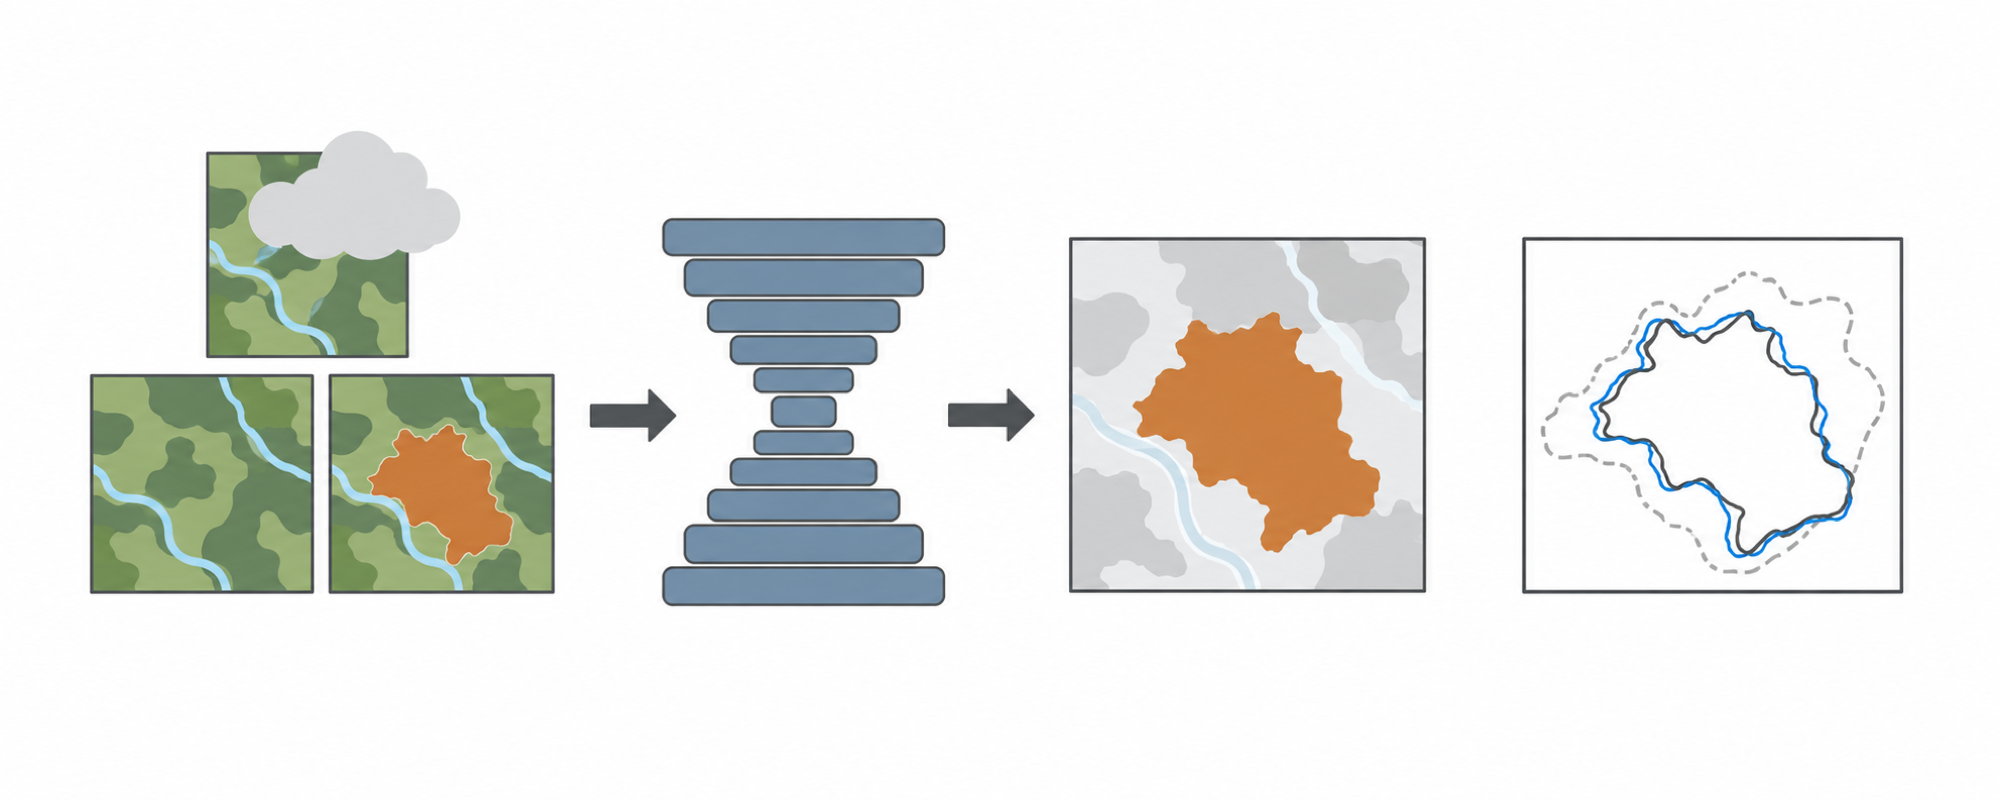
\includegraphics[width=\linewidth]{figures/ch10/ch10-03-composition-a-narrative.png}};
\begin{scope}[x={(img.south east)},y={(img.north west)}]
  \tikzset{stglbl/.style={font=\sffamily\scriptsize\bfseries,text=BookInk,fill=white,fill opacity=0.90,text opacity=1,inner sep=1.5pt,align=center}}
  \node[stglbl] at (0.165,0.16) {(1) Input pair \& cloud limit};
  \node[stglbl] at (0.40,0.16) {(2) Segmentation network};
  \node[stglbl] at (0.62,0.16) {(3) Burned-area map};
  \node[stglbl] at (0.855,0.16) {(4) Edge comparison};
\end{scope}
\end{tikzpicture}
\caption{Composition A: left-to-right narrative. Input, model, output, and finding occupy four stages from left to right; reading starts in one place and ends on the comparison. The cloud tile puts ``needs cloud-free views'' where every reader passes. Base art generated by an image model; all image tiles are schematic.}\label{fig:ch10-03}
\end{figure}

Inspecting the actual artwork in Figure~\ref{fig:ch10-03}: all four stages are present; the pre- and post-fire tiles on the left share matching river bends with the cloud-obscured tile above them; the middle shows a single-column hourglass of 10 rounded rectangles; Stages (1)$\rightarrow$(2) and (2)$\rightarrow$(3) are linked by two identical dark-gray filled arrows with no arrow between (3) and (4); and the comparison box on the right separates the dark-gray solid line, the closely tracking blue solid line, and the deviating light-gray dashed line. Three minor deviations also appear: the cloud is drawn fairly large and extends slightly above its small tile frame; the four stages are not strictly equal in width (the input pair reaches about $x=0.28$, and the output tile is larger than one input tile); and fills show slight tonal variation rather than pure flat color. Run 2 shrank the cloud neatly, but dropped the dark-gray outlines around the hourglass and lost geometric consistency across tiles, so Run 1 was selected.

Now examine \textbf{Candidate B (central figure)}: Stage (3)'s burned-area map is enlarged at the center, while the pre-fire tile, post-fire tile (with its cloud-limit tile), segmentation network, and boundary comparison inset sit at the four corners, connected to the center by plain gray lines without arrowheads. Key parts of the English prompt are shown below (full version in the \texttt{cases/} directory of the book repository):

\begin{Prompt}
Graphical abstract base art, wide banner, aspect ratio 5:2 (2000 x 800 px),
pure white background, flat 2D vector illustration, thin dark gray outlines.
ABSOLUTELY NO TEXT: no letters, words, numbers, symbols, labels or title.
Central composition. In the exact center, one large square top-down schematic
map tile (about 70% of image height) of a landscape patch in very pale gray with
a crisp warm brown-orange burned-area polygon and a thin pale-blue river line.
Around it, four small elements, each about one quarter the size of the center:
- upper left: small tile of the same patch in muted green vegetation (before);
- lower left: small tile of the same patch with a warm brown-orange area (after),
  and next to it an even smaller tile partly covered by a flat light gray cloud;
- upper right: small blue-gray hourglass shape of stacked rounded rectangles;
- lower right: small square inset with three boundary lines: dark gray solid,
  blue solid closely following it, light gray dashed clearly deviating.
Thin plain gray connector lines without arrowheads run from each small element
toward the central tile. Do not draw: flames, smoke, globes, satellites, clocks.
\end{Prompt}

The central composition took three runs, and the two rejected runs expose common pitfalls of multi-element radial layouts: in Run 1, the central map retained green vegetation instead of a pale-gray background and the network split into two columns; Run 2 fixed the pale-gray center and single-column hourglass, but attached the lower-left connector line directly to the tiny cloud-covered tile, leaving the main post-fire input tile disconnected; only in Run 3---after specifying exact connector attachment points and detaching the cloud tile---did we obtain a structurally sound Candidate B (Figure~\ref{fig:ch10-04}).

\begin{figure}[htbp]\centering
\begin{tikzpicture}
\node[anchor=south west,inner sep=0] (img) at (0,0) {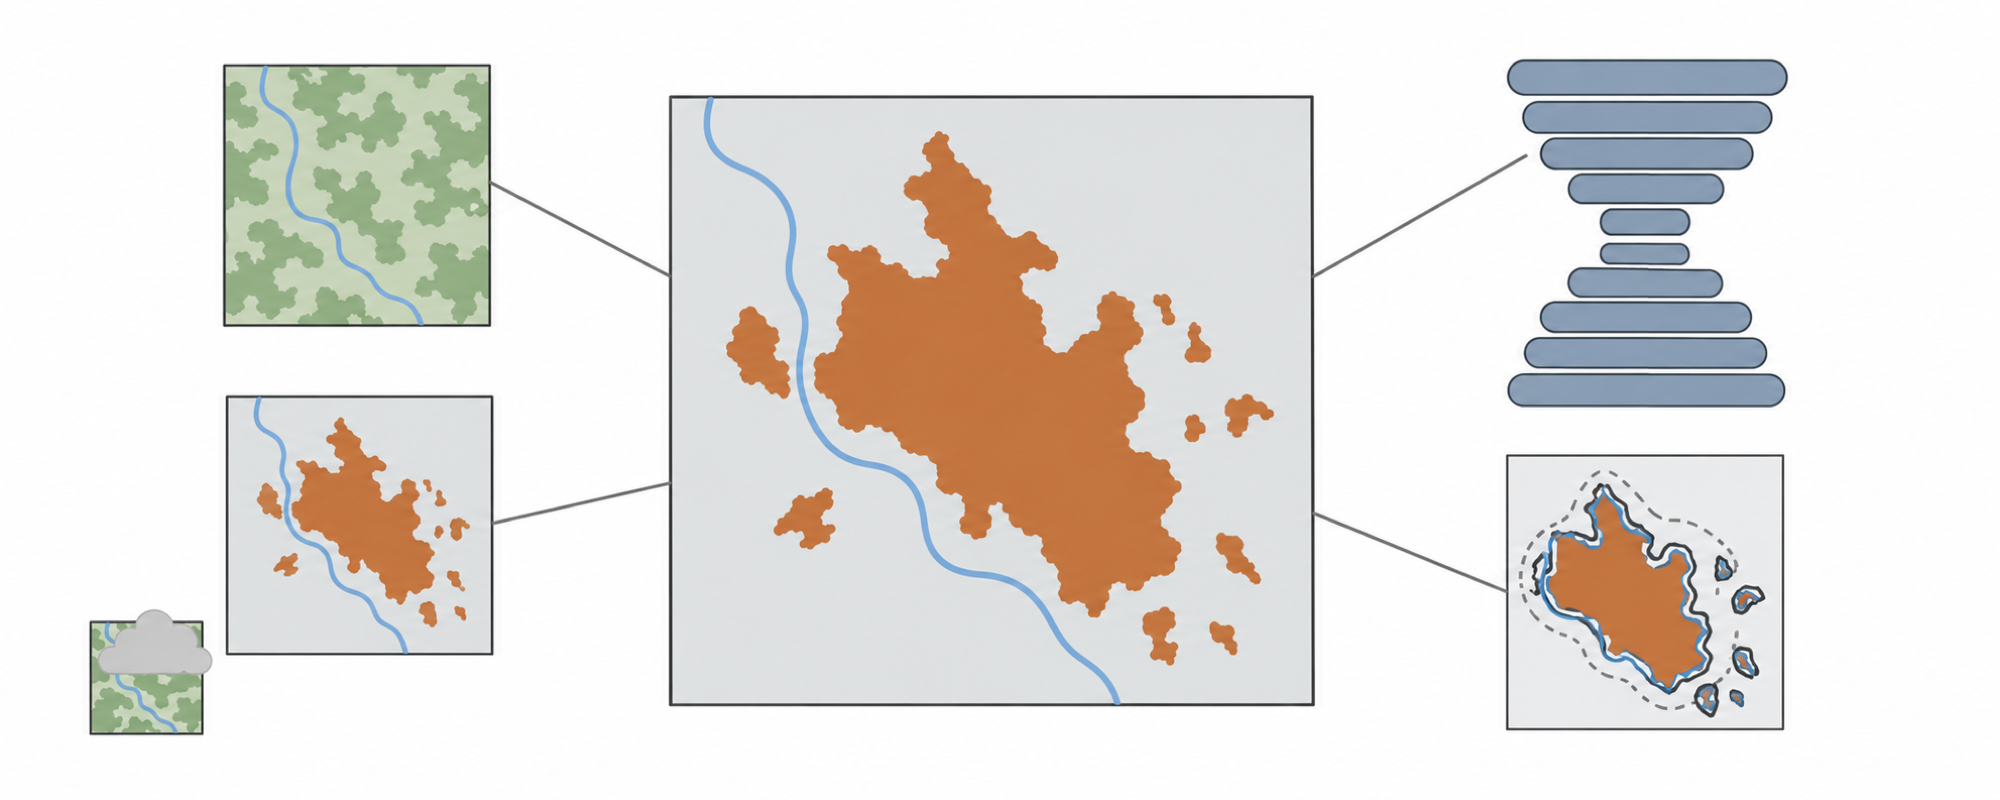
\includegraphics[width=\linewidth]{figures/ch10/ch10-04-composition-b-central.png}};
\begin{scope}[x={(img.south east)},y={(img.north west)}]
  \tikzset{stglbl/.style={font=\sffamily\scriptsize\bfseries,text=BookInk,fill=white,fill opacity=0.90,text opacity=1,inner sep=1.2pt,align=center}}
  \node[stglbl] at (0.175,0.54) {(1) Pre-fire tile};
  \node[stglbl] at (0.175,0.11) {(1) Post-fire \& cloud tiles};
  \node[stglbl] at (0.82,0.45) {(2) Segmentation network};
  \node[stglbl] at (0.49,0.05) {(3) Burned-area map (center)};
  \node[stglbl] at (0.82,0.04) {(4) Edge comparison};
\end{scope}
\end{tikzpicture}
\caption{Composition B: central figure. Same content as Figure~\ref{fig:ch10-03}. The central map draws the eye, but in a $5:2$ banner the surrounding elements shrink, and the comparison with the threshold method retreats to the lower-right corner---the first thing lost at thumbnail size. For a $1200\ \text{px}$ square format this layout adapts more easily.}\label{fig:ch10-04}
\end{figure}

Figure~\ref{fig:ch10-04} also shows the limits of a central layout in a $5:2$ banner: the central map takes up about $77\%$ of canvas height, pushing surrounding elements to the sides; the upper-right hourglass is oversized, whereas the lower-right comparison inset carrying the finding is squeezed into a corner where its small patches and three contour lines blur together when scaled down; and the cloud-limit tile retreats to the far lower-left corner. Table~\ref{tab:ch10-04-ab} compares the two compositions systematically.

\begin{table}[htbp]\centering\footnotesize
\setlength{\tabcolsep}{3pt}
\renewcommand{\arraystretch}{1.15}
\caption{Comparison between Candidate A (left-to-right narrative) and Candidate B (central figure).}\label{tab:ch10-04-ab}
\begin{tabularx}{\linewidth}{@{}>{\raggedright\arraybackslash}p{25mm}YY@{}}
\toprule
\textbf{Criterion} & \textbf{Candidate A: Left-to-right narrative (Figure~\ref{fig:ch10-03})} & \textbf{Candidate B: Central figure (Figure~\ref{fig:ch10-04})} \\
\midrule
Reading entry point & Unique (pre-/post-fire pair at far left) & Eye lands on the center map first; inputs and comparison scatter around four corners \\
Endpoint on ``Finding''? & Yes (boundary comparison inset at far right) & Center map is the output; the ``closer than threshold'' comparison is pushed to the lower-right corner \\
$5:2$ banner fit & Good; four horizontal stages leave top and bottom text bands & Center map occupies $\approx 77\%$ of height, leaving little room for full-width text bands \\
$200\ \text{px}$ high thumbnail & Stage icons and main contours remain distinguishable & Surrounding small elements and fine lower-right comparison lines blur first \\
Scope-limit placement & Cloud icon above input pair + bottom full-width text line, right on the reading path & Cloud icon pushed to the far lower-left corner, easy to overlook \\
If adapted to $1200\ \text{px}$ square & Must fold into two rows (Z-shaped reading path) & Four-corner hub-and-spoke topology fits a square naturally \\
\midrule
\textbf{Conclusion} & \textbf{Select A} (target is an Elsevier $5:2$ banner) & Keep as a backup for square-format venues \\
\bottomrule
\end{tabularx}
\end{table}

Both candidates look clean, but the choice rests on aspect ratio, reading entry and exit points, and limit visibility at thumbnail scale---not subjective aesthetics. If the paper were later reformatted for a $1200 \times 1200\ \text{px}$ square format, Candidate B would adapt more naturally.

\section{Over-Claiming: When the Image Says More Than the Paper}

Suppose a co-author looks at Candidate A, says ``It looks too plain---make it dramatic and highlight AI's early-warning capability and global significance,'' and submits the following counter-example prompt:

\begin{Prompt}
Deliberately over-dramatic graphical abstract base art for a teaching
counter-example, wide banner, aspect ratio 5:2 (2000 x 800 px).
Dark blue gradient background with glowing accents.
Left: a photorealistic satellite-style top-down view of a forest with a bright
red-orange active fire front and thick gray smoke plumes.
Center: a glowing glossy 3D "AI brain" made of circuit lines, with light rays.
Right: a 3D Earth globe covered by a bright grid, with several red flame icons
on it, a red triangular alarm icon, and an alarm clock.
Glossy, cinematic, high contrast, lens flare.
NO TEXT: no letters, no words, no numbers, no symbols, no labels.
Leave a dark empty band across the top 18% for a headline.
\end{Prompt}

Generating this counter-example base image revealed an important detail: even though the prompt specified \texttt{NO TEXT}, Run 1 drew numerals $1\text{--}12$ on the clock dial and an exclamation mark inside the red triangle, and Run 2 still left a short vertical tick mark at the 12 o'clock position resembling the digit ``1.'' Only Run 3---after we required a blank dial with only two hands and an empty warning triangle---eliminated all built-in characters. On top of the Run 3 base image, we overlaid typical exaggerated headlines, a percentage badge, and a prediction slogan in TikZ (along with a ``fictional exaggerated counter-example'' watermark to prevent misuse if screenshotted), marking seven over-claims as \textbf{O1--O7} (Figure~\ref{fig:ch10-05}).

\begin{figure}[htbp]\centering
\begin{tikzpicture}
\node[anchor=south west,inner sep=0] (img) at (0,0) {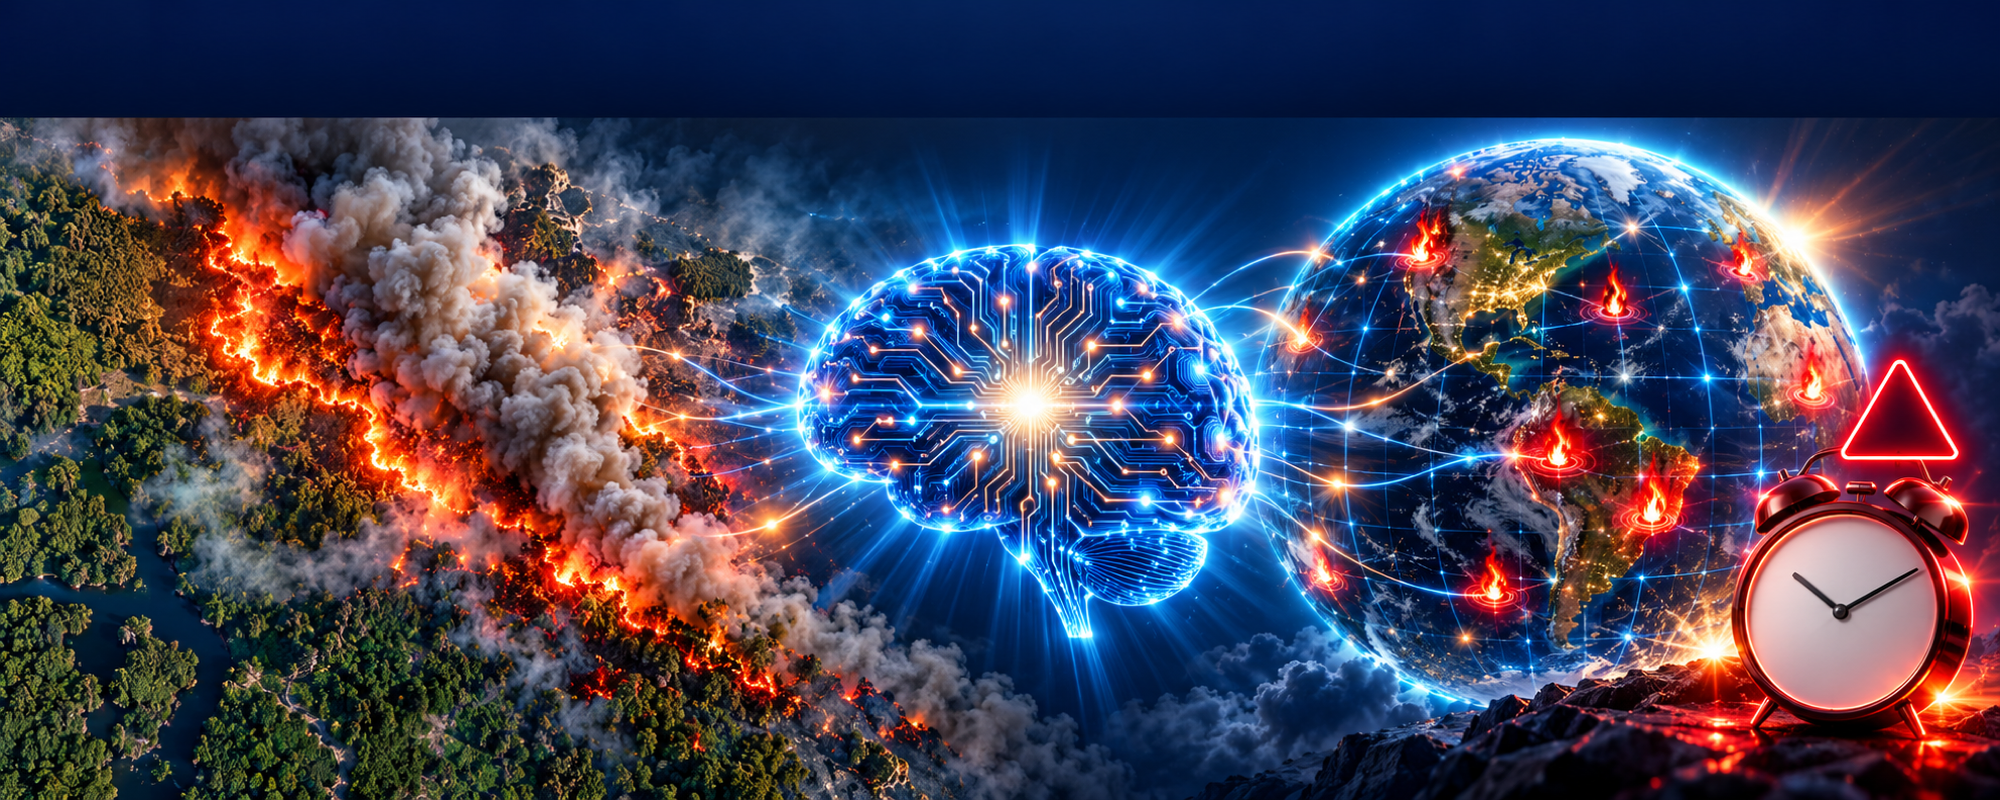
\includegraphics[width=\linewidth]{figures/ch10/ch10-05-overclaim.png}};
\begin{scope}[x={(img.south east)},y={(img.north west)}]
  \tikzset{
    overtxt/.style={font=\sffamily\bfseries,text=white,align=center},
    badmark/.style={draw=red!85!black,very thick,rounded corners=2pt,fill=white,fill opacity=0.92,text opacity=1,text=red!85!black,font=\sffamily\bfseries\scriptsize,inner sep=1.5pt}
  }
  \node[overtxt,font=\sffamily\normalsize\bfseries] at (0.52,0.92) {Real-time global wildfire AI};
  \node[font=\sffamily\scriptsize\bfseries,text=yellow!90!white,fill=black!65,inner sep=1.5pt,rounded corners=1pt] at (0.50,0.81) {[Fictional exaggerated counter-example $\cdot$ not a real study]};
  \node[overtxt,font=\sffamily\large\bfseries,text=yellow!95!white,fill=black!55,inner sep=2pt,rounded corners=2pt] at (0.50,0.45) {99\% accuracy};
  \node[overtxt,font=\sffamily\footnotesize\bfseries,fill=red!75!black,inner sep=2pt,rounded corners=2pt] at (0.72,0.12) {Predicts fires before they start};
  \node[badmark] at (0.09,0.34) {O1};
  \node[badmark] at (0.19,0.50) {O2};
  \node[badmark] at (0.77,0.56) {O3};
  \node[badmark] at (0.91,0.24) {O4};
  \node[badmark] at (0.37,0.45) {O5};
  \node[badmark] at (0.24,0.92) {O6};
  \node[badmark] at (0.27,0.70) {O7};
\end{scope}
\end{tikzpicture}
\caption{Counter-example: an over-claiming graphical abstract (fictional). A photographic ``satellite image,'' a fire front, a globe, an alarm clock, and an unqualified percentage inflate burned-area mapping into observational evidence, active-fire detection, global coverage, forecasting, and universal accuracy. The headline and number are deliberately exaggerated fiction, not results. Base art generated by an image model.}\label{fig:ch10-05}
\end{figure}

Table~\ref{tab:ch10-05-overclaim} breaks down the seven over-claims (O1--O7) in Figure~\ref{fig:ch10-05} and their conservative fixes.

\begin{table}[htbp]\centering\footnotesize
\setlength{\tabcolsep}{3pt}
\renewcommand{\arraystretch}{1.12}
\caption{Breakdown and conservative correction of the seven over-claims (O1--O7) in Figure~\ref{fig:ch10-05}.}\label{tab:ch10-05-overclaim}
\begin{tabularx}{\linewidth}{@{}c>{\raggedright\arraybackslash}p{25mm}>{\raggedright\arraybackslash}p{25mm}>{\raggedright\arraybackslash}p{26mm}Y@{}}
\toprule
\textbf{\#} & \textbf{Over-claiming element} & \textbf{What it implies} & \textbf{What the paper supports} & \textbf{Conservative correction} \\
\midrule
O1 & Photorealistic overhead forest ``image'' & Real satellite observational photo & Schematic pre-/post-fire pair; target is burned ground & Revert to flat schematic tiles; note ``schematic, not real satellite data'' in caption \\
O2 & Bright fire front, flame icons, and red warning triangle & Active fire detection and emergency alerting & Post-fire burned-area mapping & Delete fire front, flames, and alarm; draw burned area as a static warm brown-orange polygon \\
O3 & Globe with glowing global grid & Applicable globally across ecoregions & Tested on held-out fires; cross-ecoregion transfer unverified & Delete globe and grid; draw a single schematic patch and state test scope \\
O4 & Alarm clock and ``Predicts fires before they start'' & Forecasts fire ignition before it starts & Maps burned area once first cloud-free post-fire image arrives & Delete clock and ``predicts''; write ``from the first clear post-fire image'' \\
O5 & Large ``99\% accuracy'' badge & Universal high accuracy number & Reports closer agreement with reference edges than fixed-threshold dNBR; numbers need metric and baseline context & Delete numbers; express the comparative finding via the three-line boundary inset \\
O6 & ``Real-time global wildfire AI'' headline & Global coverage, real-time response & Bounded by satellite revisit and clouds/smoke & Change headline to ``Burned-area maps from the first clear post-fire image'' \\
O7 & Dense smoke pierced by AI light beams, with cloud limit omitted & Unaffected by clouds or smoke; all-weather penetration & Optical agreement drops under clouds or smoke; requires cloud-free views & Remove smoke-piercing beams; restore gray cloud tile at input and bottom limits line \\
\bottomrule
\end{tabularx}
\end{table}

Notice \textbf{O7} in particular: thick 3D smoke billows over the forest on the left while glowing beams from the central brain pierce straight through the smoke toward the global grid, and the ``needs cloud-free views'' cloud tile has vanished---falsely implying that optical bands penetrate thick wildfire smoke.

\begin{BookNote}
\textbf{Principle: Every icon in a graphical abstract is a declarative sentence.} Reviewers and readers read ``flames'' as ``detects active fire,'' a ``globe'' as ``works globally,'' an ``alarm clock'' as ``early warning,'' and ``beams piercing smoke'' as ``immune to cloud and smoke cover.'' During inspection, translate every visual element into a sentence and find its evidence in the paper; if you cannot find it, delete the element.
\end{BookNote}

When faced with a thoroughly derailed draft like Figure~\ref{fig:ch10-05}, do not use it as a reference image for piecemeal patching; instead, \textbf{return directly to the Candidate A base image (Figure~\ref{fig:ch10-03})} and issue a focused revision instruction:

\begin{Prompt}
Start from Draft A; do not use the dramatic version. Keep Draft A's four-stage
layout and all existing objects unchanged.
No flames, smoke plumes, red alarms, globes, alarm clocks, or photorealistic
imagery, and no numbers or text.
Make only two changes: (1) enlarge the output burned-area map tile to about 1.2
times the input tile size; (2) thicken the three boundary lines in the
comparison inset so the deviation between the light-gray dashed line and the
blue solid line stays visible when scaled down.
\end{Prompt}

\section{Final Artwork, the Thumbnail Test, and Verification}

We turn the revision instructions above into the final English base prompt (full version in the \texttt{cases/} directory of the book repository):

\begin{Prompt}
Final graphical abstract base art, wide banner, aspect ratio 5:2,
2000 x 800 px, pure white background, flat 2D vector illustration, flat fills,
uniform thin dark gray (#3A3A3A) outlines, no gradients, no shadows, no 3D.
THIS IMAGE MUST CONTAIN NO TEXT AT ALL: no letters, words, numbers, symbols.
EMPTY BANDS: keep y 0.00-0.15 (top), y 0.76-0.84 (caption strip under the four
stages) and y 0.88-1.00 (bottom) completely white.
Four stages, all objects vertically within y 0.18-0.72:
1. x 0.04-0.25: two square schematic map tiles side by side (left: muted green
   #A8C3A0 vegetation; right: same patch with #C8743C burned area), same river.
   Smaller tile partly covered by a flat light gray (#D5D5D5) cloud at upper left.
2. x 0.30-0.45: one blue-gray (#8FA3B8) hourglass of stacked rounded rectangles.
3. x 0.50-0.73: one larger square map tile in very pale gray with a crisp
   #C8743C burned-area polygon (about 1.2 times the input tiles).
4. x 0.77-0.96: a square inset with three thick boundary lines: #3A3A3A solid
   (reference), #2F6DB5 solid closely following it, #A0A0A0 dashed deviating.
Two identical #3A3A3A arrows: stage 1 -> 2, stage 2 -> 3; no arrow between 3 and 4.
\end{Prompt}

The final base artwork also took three runs: without a reference image, Run 1 split the hourglass into left and right columns forming an X-shape with weak dashed-line separation, and Run 2 fixed the network and thickened the lines but generated a different river course and burned polygon from Candidate A. In Run 3, \textbf{attaching Candidate A (Figure~\ref{fig:ch10-03}) as a visual reference} preserved Candidate A's river course, burned-area outline, single-column hourglass, and twin flow arrows while thickening the three comparison contours in Stage (4). Three minor residual deviations remain: the output square side length is about $1.6$ times a single input tile (aligning with the combined height of the stacked left tiles rather than strictly $1.2$ times), some frame bottoms reach about $y=0.75$, and empty-band RGB values fluctuate between $249$ and $255$. None of these details affects the scientific message, and all three text bands are clean.

We then overlay seven vector text elements (Table~\ref{tab:ch10-06-text}) in TikZ on the text-free base to produce the final graphical abstract (Figure~\ref{fig:ch10-06}).

\begin{table}[htbp]\centering\footnotesize
\setlength{\tabcolsep}{3pt}
\renewcommand{\arraystretch}{1.15}
\caption{Vector text layers (T1--T7) overlaid on the final graphical abstract (Figure~\ref{fig:ch10-06}).}\label{tab:ch10-06-text}
\begin{tabularx}{\linewidth}{@{}cY>{\raggedright\arraybackslash}p{30mm}>{\raggedright\arraybackslash}p{32mm}@{}}
\toprule
\textbf{\#} & \textbf{English vector text layer} & \textbf{Contribution-card role} & \textbf{Position and size tier} \\
\midrule
T1 & Burned-area maps from the first clear post-fire image & Question \& takeaway & $(0.50,0.92)$ top center; largest tier \\
T2 & Pre-/post-fire Sentinel-2 pair & Method (input) & Below Stage (1); medium (TOC-legible) \\
T3 & Segmentation network & Method (model) & Below Stage (2); medium (TOC-legible) \\
T4 & Burned-area map & Method (output) & Below Stage (3); medium (TOC-legible) \\
T5 & Closer to reference edges than dNBR threshold & Finding (comparison) & Below Stage (4); medium (TOC-legible) \\
T6 & Maps areas already burned $\cdot$ not fire detection or forecasting $\cdot$ needs cloud-free views & Limits (mandatory scope) & $(0.50,0.04)$ bottom center; small (article-page legible) \\
T7 & reference / model / threshold & Comparison legend & Below T5 in Stage (4); smallest tier \\
\bottomrule
\end{tabularx}
\end{table}

\begin{figure}[htbp]\centering
\begin{tikzpicture}
\node[anchor=south west,inner sep=0] (img) at (0,0) {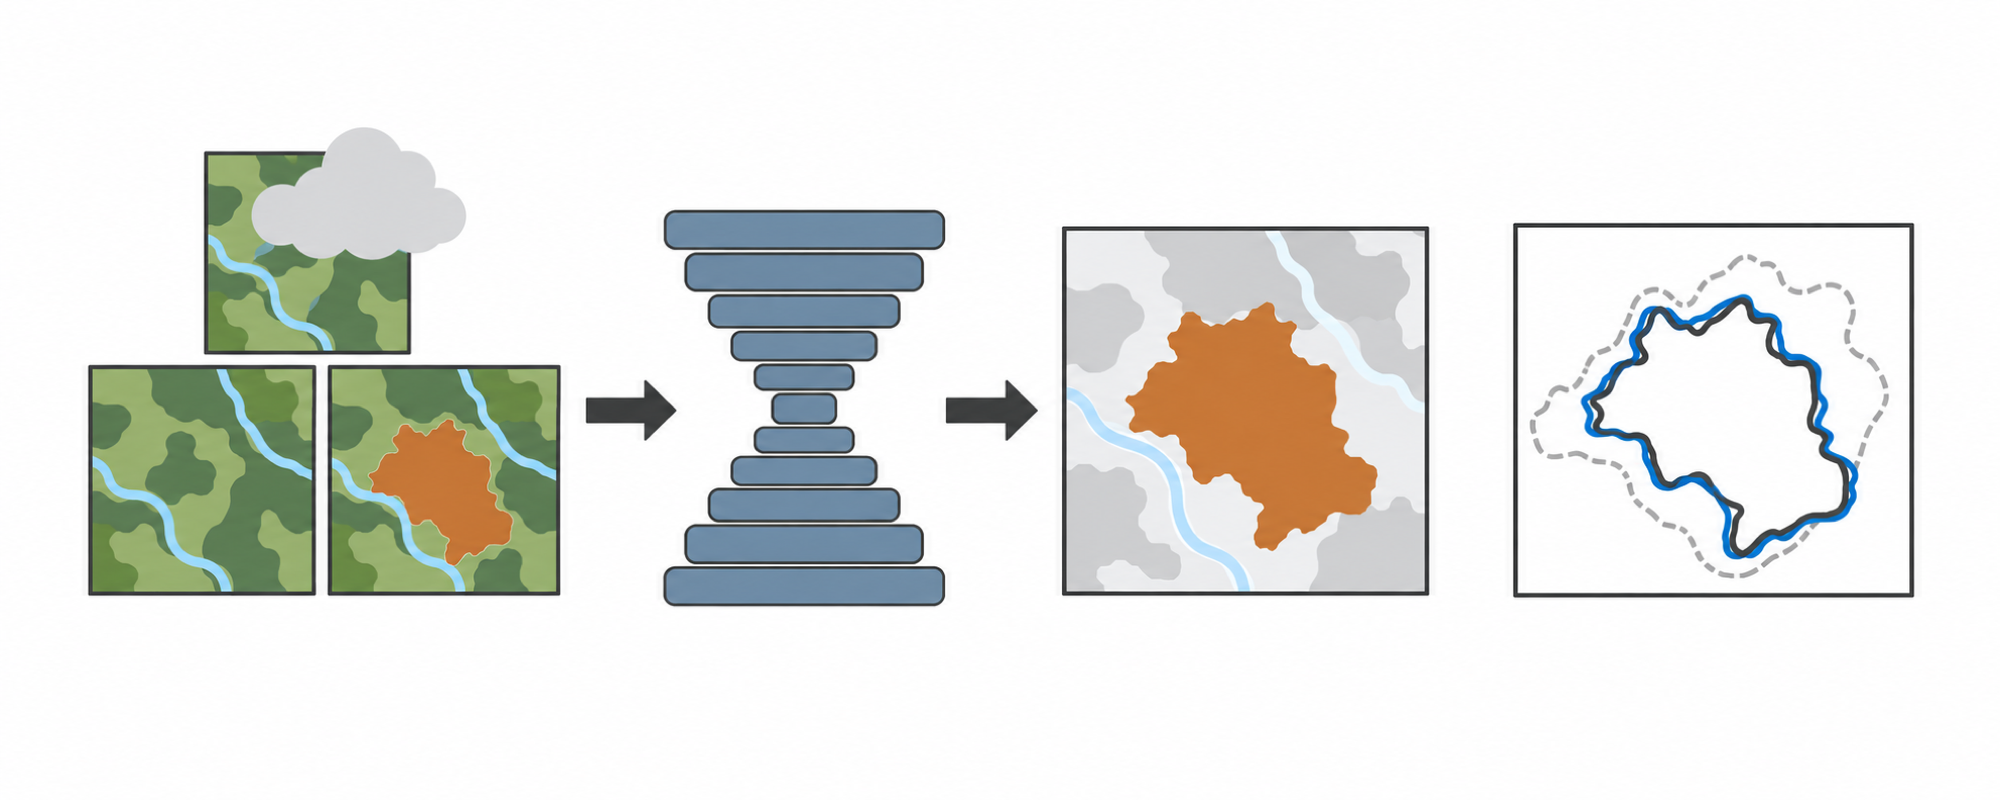
\includegraphics[width=\linewidth]{figures/ch10/ch10-06-final-base.png}};
\begin{scope}[x={(img.south east)},y={(img.north west)}]
  \tikzset{
    t1style/.style={font=\sffamily\small\bfseries,text=BookInk,align=center},
    tstg/.style={font=\sffamily\scriptsize\bfseries,text=BookInk,fill=white,fill opacity=0.90,text opacity=1,inner sep=1pt,align=center},
    t6style/.style={font=\sffamily\scriptsize,text=BookInk!90,align=center},
    t7style/.style={font=\sffamily\tiny,text=BookInk!85,align=center}
  }
  \node[t1style] at (0.50,0.92) {Burned-area maps from the first clear post-fire image};
  \node[tstg] at (0.165,0.185) {Pre-/post-fire\\[-1pt]Sentinel-2 pair};
  \node[tstg] at (0.40,0.185) {Segmentation\\[-1pt]network};
  \node[tstg] at (0.62,0.185) {Burned-area map};
  \node[tstg] at (0.855,0.185) {Closer to reference edges\\[-1pt]than dNBR threshold};
  \node[t7style] at (0.855,0.105) {reference / model / threshold};
  \node[t6style] at (0.50,0.04) {Maps areas already burned $\cdot$ not fire detection or forecasting $\cdot$ needs cloud-free views};
\end{scope}
\end{tikzpicture}
\caption{Final graphical abstract for the teaching case. From left: a pre-/post-fire image pair, the segmentation network, the burned-area map, and a schematic comparison with reference edges. The bottom line states the limits. All image tiles are flat schematics, \textbf{not real satellite data}; the study is a fictional teaching scenario, not a published result. Base art was generated by an image model; text is typeset with TikZ.}\label{fig:ch10-06}
\end{figure}

The final step turns ``Is it still legible at table-of-contents size?'' into a reproducible \textbf{thumbnail test}. When a $2000 \times 800\ \text{px}$ image is scaled to Elsevier's $200\ \text{px}$ high TOC window ($500 \times 200\ \text{px}$), linear dimensions shrink to one-quarter. Stage names set at $\approx 36\ \text{px}$ font height scale to $\approx 9.0\ \text{px}$ tall and remain legible; set at $14\ \text{px}$, they shrink to $\approx 3.5\ \text{px}$ and blur together (Figure~\ref{fig:ch10-07}). In the top row of Figure~\ref{fig:ch10-07}, setting the long fourth label on a single line at $36\ \text{px}$ causes it to collide with Stage 3 and clip at the right border---which is why our TikZ overlay in Figure~\ref{fig:ch10-06} wraps longer labels onto two lines. Essential scope limits must also sit inside the image like T6 (with the cloud icon), not just in an external caption.

\begin{figure}[htbp]\centering
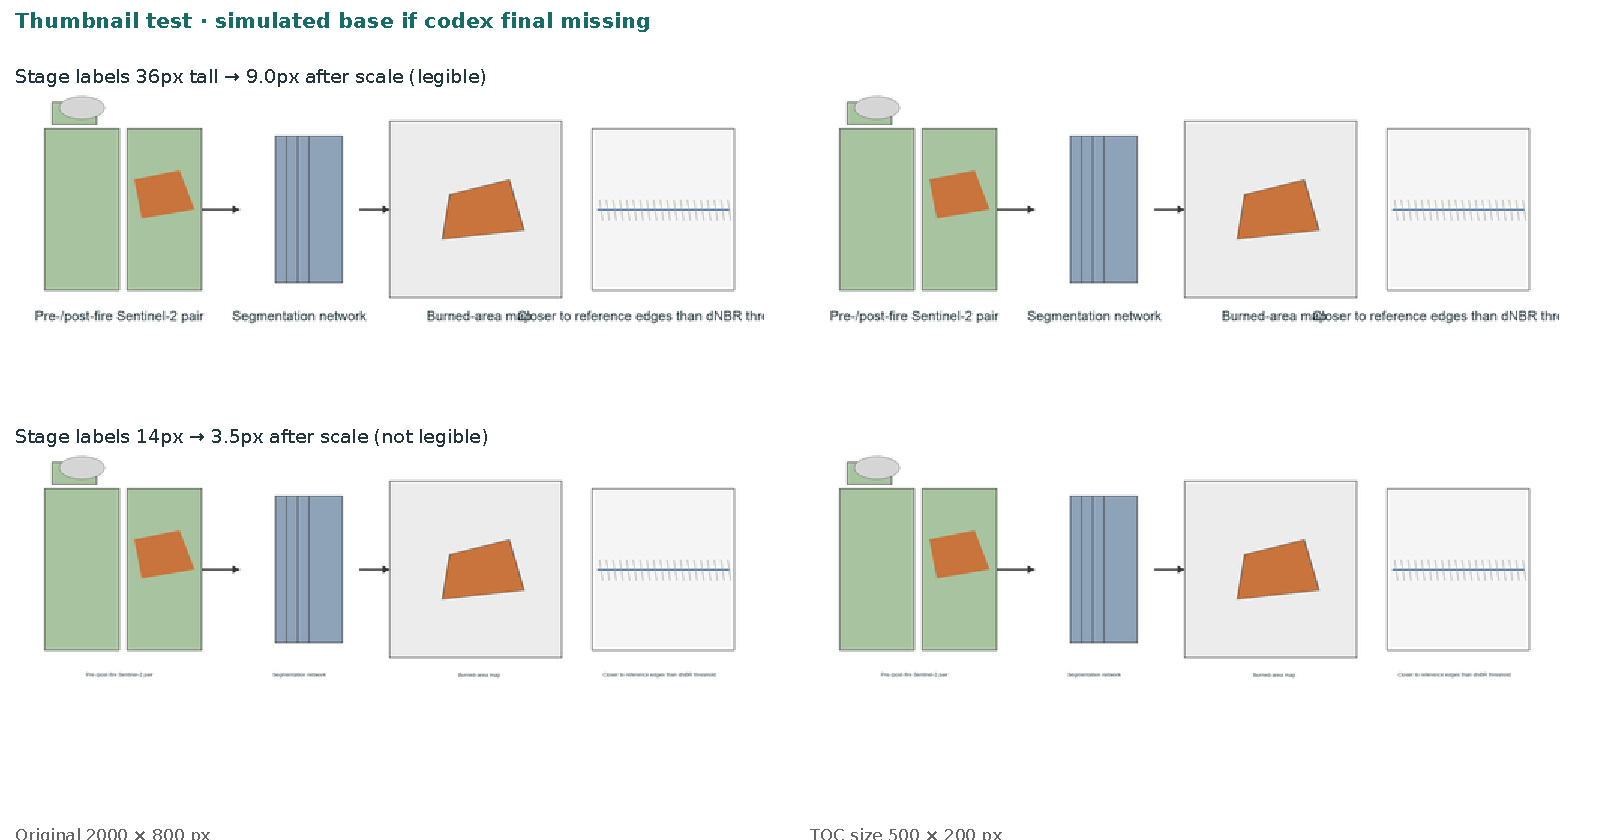
\includegraphics[width=\linewidth]{figures/ch10/ch10-07-thumbnail-test-en.pdf}
\caption{Thumbnail test. The graphical abstract scaled to about $200\ \text{px}$ high---the TOC display height mentioned in Elsevier's guidelines---shown at actual pixels (tested here on the same $2000 \times 800\ \text{px}$ simulated layout base while varying only stage-label font height). Top: stage names at $36\ \text{px}$ height scale to $9.0\ \text{px}$ and remain legible. Bottom: the same image with $14\ \text{px}$ stage names scales to $3.5\ \text{px}$ and becomes unreadable. The limits line is small in the thumbnail but readable on the article page.}\label{fig:ch10-07}
\end{figure}

\section{Walk-Through of the Complete Chapter Case}

In this chapter case, we started from a fictional teaching abstract and completed journal rule verification (Figure~\ref{fig:ch10-01}), four-line contribution card distillation (Table~\ref{tab:ch10-02-card}), PDF-to-prompt boundary auditing (Figure~\ref{fig:ch10-02}, Table~\ref{tab:ch10-03-compare}), A/B composition comparison (Figures~\ref{fig:ch10-03} and \ref{fig:ch10-04}, Table~\ref{tab:ch10-04-ab}), over-claim counter-example deconstruction (Figure~\ref{fig:ch10-05}, Table~\ref{tab:ch10-05-overclaim}), final base refinement and TikZ vector lettering (Figure~\ref{fig:ch10-06}), and the $200\ \text{px}$ thumbnail test (Figure~\ref{fig:ch10-07}). The nine pre-delivery verification checks are recorded in Table~\ref{tab:ch10-07-verify}.

\begin{table}[htbp]\centering\footnotesize
\setlength{\tabcolsep}{3pt}
\renewcommand{\arraystretch}{1.15}
\caption{Nine-item verification table (C1--C9) for the final teaching-case graphical abstract (Figure~\ref{fig:ch10-06}).}\label{tab:ch10-07-verify}
\begin{tabularx}{\linewidth}{@{}c>{\raggedright\arraybackslash}p{26mm}>{\raggedright\arraybackslash}p{32mm}Y@{}}
\toprule
\textbf{\#} & \textbf{Check item} & \textbf{Verification method} & \textbf{Recorded result} \\
\midrule
C1 & All four contribution-card rows in figure & Point to the element for each row & Question and Method map to Stages (1)--(3) and T1--T4; Finding maps to Stage (4) and T5; Limits map to upper-left cloud tile and bottom T6 phrase \\
C2 & No elements beyond the paper & Translate each icon into a sentence and check against abstract & All objects match the brief's schematic elements; no flames, globes, alarm clocks, or percentage numbers \\
C3 & No numbers, data plots, or photo-textured imagery & Zoom check of textures and graphic categories & No numbers or data plots; map tiles are flat schematics (fills have slight tonal variation; caption states ``not real satellite data'') \\
C4 & Aspect ratio and pixels & Check file properties: $5:2$, $\ge 1328 \times 531\ \text{px}$ & Delivered base art is $2000 \times 800\ \text{px}$, meeting the $5:2$ ratio and pixel floor \\
C5 & Thumbnail legibility & Figure~\ref{fig:ch10-07} test: stage names legible at $200\ \text{px}$ height & Stage names set at $\approx 36\ \text{px}$ height scale to $\approx 9.0\ \text{px}$ at $200\ \text{px}$ height and remain recognizable \\
C6 & No pseudo-text in base art & Full-size zoom inspection & Selected base image shows no letters, digits, or pseudo-text (earlier counter-example runs with dial digits and ticks were rejected) \\
C7 & Chinese and English editions differ only in text layer & Compare base-image file hashes & Both editions share the same text-free base file and switch only the TikZ text layer per Table~\ref{tab:ch10-06-text} \\
C8 & Journal rules re-checked before submission & Log target journal URL and access date & Logged Elsevier general guidelines URL and October 2026 access date; re-verify on the target journal page before upload \\
C9 & PDF-to-prompt scope and raw output archived & Check local figure archive records & When using \sdtool{graphical-abstract-maker}, archive the 5-page scope, verbatim prompt, and comparison table together \\
\bottomrule
\end{tabularx}
\end{table}

\section{What AI Can and Cannot Do at This Stage}

The division of labor between AI tools and the author across graphical-abstract production is summarized in Table~\ref{tab:ch10-08-ai}.

\begin{table}[htbp]\centering\footnotesize
\setlength{\tabcolsep}{3pt}
\renewcommand{\arraystretch}{1.15}
\caption{What AI can do, what AI cannot do, and what the author must verify when making a graphical abstract.}\label{tab:ch10-08-ai}
\begin{tabularx}{\linewidth}{@{}>{\raggedright\arraybackslash}p{18mm}YYY@{}}
\toprule
\textbf{Stage} & \textbf{What AI (\scidraw{}, etc.) can do} & \textbf{What AI cannot do} & \textbf{What the author must verify} \\
\midrule
Reading paper & Graphical-abstract tool reads first 5 PDF pages ($\le 6{,}000$ chars) and drafts a $60\text{--}110$-word visual prompt & Understand full paper; decide which finding matters most; guarantee scope limits are kept & Log reading scope and raw output; compare line by line with contribution card and restore limits \\
Distilling contribution & Shorten abstract sentences; list candidate visual objects & Decide core contribution; judge whether claim strength matches evidence & Check that every row maps to a source sentence and verbs like ``improves,'' ``solves,'' or ``predicts'' do not overreach \\
Composition & Generate multiple candidates of one layout; generate a second layout on request & Propose reasoned alternative layouts and explain trade-offs automatically (batch outputs are random variants) & Write two layouts explicitly; compare by ratio, reading path, thumbnail legibility, and limit visibility \\
Base generation & Flat schematic style, text-free base art, empty bands (with stochastic variation) & Guarantee no pseudo-text, exact coordinates, or that schematic tiles are not read as real data & Zoom to check for pseudo-text; keep imagery schematic and state ``not real data'' in caption \\
Revision & Modify using a prior image as reference per instructions & Lock objects; guarantee only target spot changes & Re-run full verification after each edit (see Chapter 11) \\
Text & (Not recommended) generate text in image & Reliable spelling and alignment & Overlay text in TikZ or layout software; proofread word by word \\
Delivery & Export image files & Know target journal's current rules & Check target journal's live page for ratio, pixels, fonts, and format; log date and run thumbnail test \\
Integrity & --- & Judge whether an icon is an over-claim & Translate every element into a sentence and verify its basis in the paper \\
\bottomrule
\end{tabularx}
\end{table}

\section{Chapter Checklist}

\begin{itemize}
\item Opened the target journal's \textbf{current} graphical-abstract page and logged the URL, access date, ratio, pixel floor, fonts, and file formats.
\item Verified that all four contribution-card rows (Question / Method / Finding / Limits) map to original sentences in the paper without inflating claim strength.
\item If PDF-to-prompt was used: archived the reading scope (first 5 pages) and raw output, compared line by line with the contribution card, and restored the limits.
\item Created at least two \textbf{explicitly reasoned} composition candidates and selected between them by aspect ratio, reading start and end points, thumbnail legibility, and limit placement.
\item Confirmed that every icon translates into a sentence supported by the paper, with no flames, globes, alarm clocks, or standalone numbers claiming more than proved.
\item Kept schematic imagery free of photorealistic texture; if real imagery is used, documented source, license, and processing.
\item Checked that base art contains no pseudo-text, overlaid all labels in a vector layer, proofread every word, and kept total word count low.
\item Verified that stage names remain legible and reading order stays clear at TOC thumbnail height (such as $200\ \text{px}$ high).
\item Confirmed that Chinese and English editions differ only in the overlaid text layer.
\item Logged tools, prompts, generation counts, and manual edits in the figure archive.
\end{itemize}

\section{Exercises}

\begin{enumerate}
\item \textbf{(Contribution card: pen and paper.)} Pick a recent paper in your field, read only the abstract and conclusion, and write a four-line contribution card; then read the full Results section and revise the ``Finding'' and ``Limits'' rows. Compare the two versions and identify which phrasing in the first version would have produced an over-claim in a graphical abstract.
\item \textbf{(Hands-on with \scidraw{}: comparing PDF-to-prompt output.)} Upload the PDF of your own paper (or the paper from Exercise 1) to \scidraw{}'s graphical-abstract tool (\sdtool{graphical-abstract-maker}) and save the returned visual prompt. Build a comparison table recording whether each row of your contribution card was ``preserved,'' ``dropped,'' or ``inflated.'' Write a revised generation prompt, generate a candidate image, and complete the Chapter Checklist.
\item \textbf{(Changing format.)} Adapt this chapter's final graphical abstract ($5:2$) to a $1200 \times 1200\ \text{px}$ square format: sketch the layout, explain whether you would fold Candidate A into two rows or use Candidate B's central figure, show where the scope limits would sit, and explain how the thumbnail test should be adjusted.
\end{enumerate}

\section*{References}

\begin{itemize}
\item American Chemical Society. \textit{The Journal of Organic Chemistry} Author Guidelines. \url{https://researcher-resources.acs.org/publish/author_guidelines?coden=joceah} (accessed 2026-10-29).
\item American Chemical Society. \textit{Langmuir} Author Checklist. \url{https://pubs.acs.org/page/langd5/submission/author-checklist} (accessed 2026-10-29).
\item Cell Press. Attract readers at a glance with your Graphical Abstract. \url{https://crosstalk.cell.com/blog/attract-readers-at-a-glance-with-your-graphical-abstract} (accessed 2026-10-29).
\item Cell Press. \textit{Cell Reports} Final File Requirements. \url{https://www.cell.com/pb-assets/journals/EM/MasterFFCs/CELREPFFC-1750868285900.pdf} (accessed 2026-10-29).
\item Chuvieco E, Mouillot F, van der Werf GR, et al. Historical background and current developments for mapping burned area from satellite Earth observation. \textit{Remote Sensing of Environment}. 2019;225:45--64. \url{https://doi.org/10.1016/j.rse.2019.02.013}
\item Elsevier. Graphical abstracts --- Author tools and resources. \url{https://www.elsevier.com/researcher/author/tools-and-resources/graphical-abstract} (accessed 2026-10-29).
\item Giglio L, Boschetti L, Roy DP, Humber ML, Justice CO. The Collection 6 MODIS burned area mapping algorithm and product. \textit{Remote Sensing of Environment}. 2018;217:72--85. \url{https://doi.org/10.1016/j.rse.2018.08.005}
\item Ibrahim AM, Lillemoe KD, Klingensmith ME, Dimick JB. Visual abstracts to disseminate research on social media: a prospective, case-control crossover study. \textit{Annals of Surgery}. 2017;266(6):e46--e48. \url{https://doi.org/10.1097/SLA.0000000000002277}
\item Knopp L, Wieland M, R\"attich M, Martinis S. A deep learning approach for burned area segmentation with Sentinel-2 data. \textit{Remote Sensing}. 2020;12(15):2422. \url{https://doi.org/10.3390/rs12152422}
\item Pferschy-Wenzig E-M, Pferschy U, Wang D, Mocan A, Atanasov AG. Does a graphical abstract bring more visibility to your paper? \textit{Molecules}. 2016;21(9):1247. \url{https://doi.org/10.3390/molecules21091247}
\item Roy DP, Huang H, Boschetti L, et al. Landsat-8 and Sentinel-2 burned area mapping --- a combined sensor multi-temporal change detection approach. \textit{Remote Sensing of Environment}. 2019;231:111254. \url{https://doi.org/10.1016/j.rse.2019.111254}
\end{itemize}

% TODO: 1) Live test output from uploading `teaching-paper.pdf` to SciDraw AI `/graphical-abstract-maker` (`provenance/ch10/pdf-prompt.txt`) remains to be captured and archived;
% TODO: 2) `figures/ch10/ch10-07-thumbnail-test-en.pdf` currently uses the script's built-in simulated base art (`simulated_base: true`); regenerate after wiring in the composited `ch10-06-final-base.png` final figure;
% TODO: 3) The main Cell Press figure guidelines page (`https://www.cell.com/figureguidelines`), previously blocked by access verification, and the ACS general graphics guideline clause on minimum 8 pt type remain to be manually verified against the original web pages.
